\documentclass[12pt]{article}

\usepackage{sbc-template}
\usepackage{graphicx,url}
\usepackage[utf8]{inputenc}
\usepackage[brazil]{babel}
\usepackage{multirow}
\usepackage{amsmath}
\usepackage{xcolor}
\usepackage{pbox}

\newcommand{\lembrete}[1]{{\color{blue}{#1}}}

\newcommand{\aspas}[1]{``{#1}''}
     
\sloppy

\title{Relatório da implementação do Robo}

\author{Gustavo José Neves da Silva\inst{1}\\Wilton Jaciel Loch\inst{1}}

\address{Departamento de Ciência da Computação\\
  Universidade do Estado de Santa Catarina (UDESC) -- Joinville, SC -- Brasil
  \email{gustavo.neves@yandex.com, wilton.loch@hotmail.com.br}
}


\begin{document} 

\maketitle

%\begin{abstract}
%  abstract
%\end{abstract}
     
\begin{resumo}
%  Este meta-artigo descreve o estilo a ser usado na confecção de artigos e
%  resumos de artigos para publicação nos anais das conferências organizadas
%  pela SBC. É solicitada a escrita de resumo e abstract apenas para os artigos
%  escritos em português. Artigos em inglês deverão apresentar apenas abstract.
%  Nos dois casos, o autor deve tomar cuidado para que o resumo (e o abstract)
%  não ultrapassem 10 linhas cada, sendo que ambos devem estar na primeira
%  página do artigo.
O presente trabalho realizado como parte da disciplina de Inteligência Artificial
% realiza uma revisão bibliográfica dos de algoritmos de agrupamento(clustering). São descritas as diferentes abordagens que acercam os algoritmos de clustering e uma implementação baseada em grid é apresentada, bem como a metodologia utilizada e resultados obtidos.
\end{resumo}

\section{Introdução} \label{sec:Introducao}

\section{Metodologia de Desenvolvimento} \label{sec:Desenvolv}
	
\section{Descrição de Experimentos/Simulações e Resultados Obtidos} \label{sec:DescExp}

\section{Análise dos resultados obtidos} \label{sec:Results}
\begin{table}[h]
	\centering
	\begin{tabular}{|l|c|}
	\hline
	& Custo total \\ \hline
	Min. & 322.0 \\ \hline
	$1^{o}$ quartil & 393.8 \\ \hline
	Mediana & 458.0 \\ \hline
	Media & 475.4 \\ \hline
	$3^{o}$ quartil & 531.5 \\ \hline
	Máx. & 750.0 \\ \hline
	\end{tabular}
	\caption{Analise custo total}
	\label{tabela:custo}
%%	
%%"" "Min.   :322.0  "
%%"" "1st Qu.:393.8  "
%%"" "Median :458.0  "
%%"" "Mean   :475.4  "
%%"" "3rd Qu.:531.5  "
%%"" "Max.   :750.0  "
%%
\end{table}

\begin{table}[h]
	\centering
	\begin{tabular}{|l|c|}
	\hline
	& Destinos escolhidos \\ \hline
	Min. & 27.00 \\ \hline
	$1^{o}$ quartil & 28.75 \\ \hline
	Mediana & 30.00 \\ \hline
	Media & 30.65 \\ \hline
	$3^{o}$ quartil & 32.25 \\ \hline
	Máx. & 37.00 \\ \hline
	\end{tabular}
	\caption{Analise destinos escolhidos}
	\label{tabela:destinos}
%%	
%%"      V1"
%%"" "Min.   :27.00  "
%%"" "1st Qu.:28.75  "
%%"" "Median :30.00  "
%%"" "Mean   :30.65  "
%%"" "3rd Qu.:32.25  "
%%"" "Max.   :37.00  "
%%
\end{table}


\begin{table}[h]
	\centering
	\begin{tabular}{|l|c|}
	\hline
	& Num. movimentos realizados \\ \hline
	Min. & 297.0 \\ \hline
	$1^{o}$ quartil & 340.5 \\ \hline
	Mediana & 410.0 \\ \hline
	Media & 419.9 \\ \hline
	$3^{o}$ quartil & 459.0 \\ \hline
	Máx. & 651.0 \\ \hline
	\end{tabular}
	\caption{Analise movimentos realizados}
	\label{tabela:movimentos}
%%
%%"      V1"
%%"" "Min.   :297.0  "
%%"" "1st Qu.:340.5  "
%%"" "Median :410.0  "
%%"" "Mean   :419.9  "
%%"" "3rd Qu.:459.0  "
%%"" "Max.   :651.0  "
%%
\end{table}


\begin{table}[h]
	\centering
	\begin{tabular}{|l|c|}
	\hline
	& Num. nós expandidos \\ \hline
	Min. & 6219 \\ \hline
	$1^{o}$ quartil & 8916 \\ \hline
	Mediana & 11220 \\ \hline
	Media & 12006 \\ \hline
	$3^{o}$ quartil & 14764 \\ \hline
	Máx. & 21126 \\ \hline
	\end{tabular}
	\caption{Analise nós expandidos}
	\label{tabela:nosExpandidos}
%%	
%%"      V1"
%%"" "Min.   : 6219  "
%%"" "1st Qu.: 8916  "
%%"" "Median :11220  "
%%"" "Mean   :12006  "
%%"" "3rd Qu.:14764  "
%%"" "Max.   :21126  "
%%
\end{table}
\section{Conclusões e Trabalhos Futuros} \label{sec:Conclusoes}

\bibliographystyle{sbc}
\bibliography{arqReferencias}

\end{document}

%
%\section{Figures and Captions}\label{sec:figs}
%
%
%Figure and table captions should be centered if less than one line
%(Figure~\ref{fig:exampleFig1}), otherwise justified and indented by 0.8cm on
%both margins, as shown in Figure~\ref{fig:exampleFig2}. The caption font must
%be Helvetica, 10 point, boldface, with 6 points of space before and after each
%caption.
%
%\begin{figure}[ht]
%\centering
%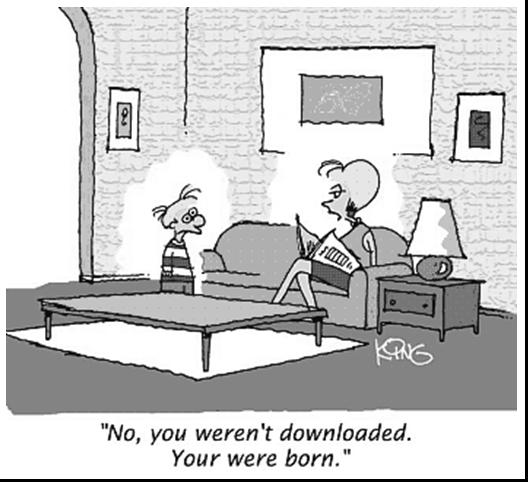
\includegraphics[width=.5\textwidth]{fig1.jpg}
%\caption{A typical figure}
%\label{fig:exampleFig1}
%\end{figure}
%
%\begin{figure}[ht]
%\centering
%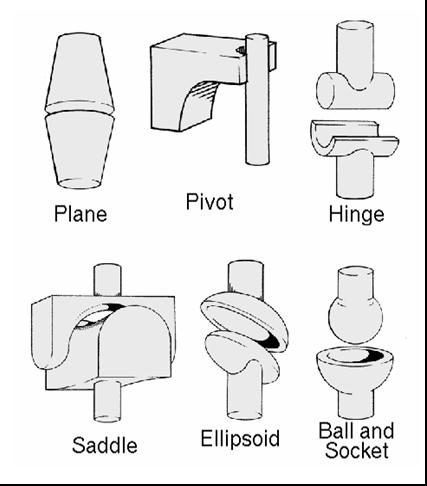
\includegraphics[width=.3\textwidth]{fig2.jpg}
%\caption{This figure is an example of a figure caption taking more than one
%  line and justified considering margins mentioned in Section~\ref{sec:figs}.}
%\label{fig:exampleFig2}
%\end{figure}
%
%In tables, try to avoid the use of colored or shaded backgrounds, and avoid
%thick, doubled, or unnecessary framing lines. When reporting empirical data,
%do not use more decimal digits than warranted by their precision and
%reproducibility. Table caption must be placed before the table (see Table 1)
%and the font used must also be Helvetica, 10 point, boldface, with 6 points of
%space before and after each caption.
%
%\begin{table}[ht]
%\centering
%\caption{Variables to be considered on the evaluation of interaction
%  techniques}
%\label{tab:exTable1}
%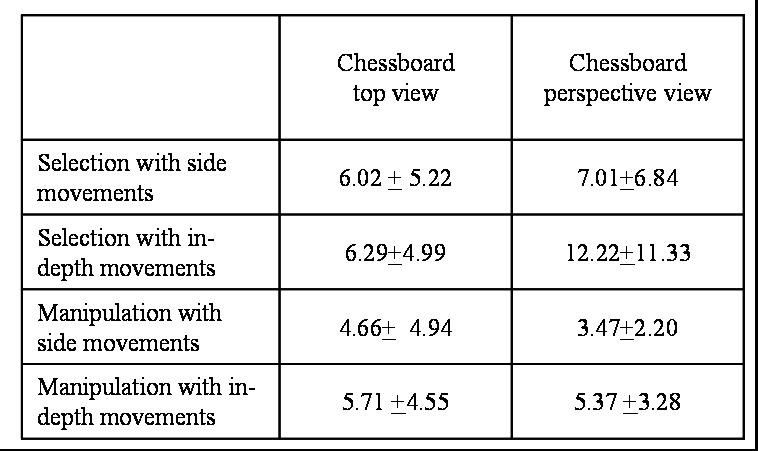
\includegraphics[width=.7\textwidth]{table.jpg}
%\end{table}
%
